\documentclass[11pt,a4paper]{article}

% ── Packages ──────────────────────────────────────────────────────────
\usepackage[utf8]{inputenc}
\usepackage[T1]{fontenc}
\usepackage{mathptmx}           % Times font
\usepackage[margin=2.2cm]{geometry}
\usepackage{amsmath,amssymb,amsfonts}
\usepackage{graphicx}
\usepackage{booktabs}
\usepackage{multirow}
\usepackage{caption}
\usepackage{subcaption}
\usepackage{xcolor}
\usepackage{hyperref}
\usepackage{algorithm}
\usepackage{algorithmic}
\usepackage{enumitem}
\usepackage{tabularx}
\usepackage{float}
\usepackage{microtype}
\usepackage{authblk}
\usepackage{setspace}

\hypersetup{
    colorlinks=true,
    linkcolor=blue!70!black,
    citecolor=blue!70!black,
    urlcolor=blue!70!black,
}

\graphicspath{{figures/}}

% ── Custom commands ───────────────────────────────────────────────────
\newcommand{\methodname}{DA-BiGRU-CNN}
\newcommand{\wpearson}{\rho_w}
\newcommand{\R}{\mathbb{R}}
\newcommand{\bx}{\mathbf{x}}
\newcommand{\bh}{\mathbf{h}}
\newcommand{\bp}{\mathbf{p}}
\newcommand{\bv}{\mathbf{v}}
\newcommand{\be}{\mathbf{e}}
\newcommand{\by}{\mathbf{y}}
\newcommand{\bW}{\mathbf{W}}
\newcommand{\bU}{\mathbf{U}}

\setlength{\parskip}{0.4em}
\setlength{\parindent}{0em}

% ══════════════════════════════════════════════════════════════════════
\begin{document}

% ── Title ─────────────────────────────────────────────────────────────
\title{%
\textbf{When Less Is More: Domain-Aware Dual-Branch Recurrent Networks\\
for Limit Order Book Mid-Price Prediction}
}

\author{Solovev Sergei}
\affil{Faculty of Computer Science, HSE University, Moscow, Russia}

\date{\small \texttt{sesesolovev@edu.hse.ru} \quad $\cdot$ \quad \url{https://sergeisolovev.com} \quad $\cdot$ \quad \url{https://github.com/SergeySolovyev}\\[0.3em]
\textbf{Code:} \url{https://github.com/SergeySolovyev/DA-BiGRU-CNN-LOB}}
\maketitle

% ── Abstract ──────────────────────────────────────────────────────────
\begin{abstract}
Predicting short-term mid-price movements from limit order book (LOB) data is a fundamental problem in quantitative finance and market microstructure research, with direct applicability to both traditional exchanges and cryptocurrency markets---including centralized exchanges (CEXs) and emerging on-chain LOB protocols in decentralized finance (DeFi). We present three contributions to this domain. \textbf{First}, we propose \methodname{}, a domain-aware dual-branch architecture that decomposes LOB features into \emph{price} and \emph{volume} information channels, processes them through dedicated bidirectional GRU encoders with shared microstructure features, and fuses temporal representations via a multi-scale convolutional bottleneck (Conv1d with kernels $k \in \{3,5,7\}$). \textbf{Second}, we provide empirical evidence for a \emph{feature sufficiency hypothesis}: a unidirectional GRU trained on 53 basic features achieves performance statistically equivalent to one trained on 219 extensively engineered features---including rolling statistics, exponential moving averages, and lag--difference features---suggesting that recurrent hidden states implicitly learn these temporal patterns. \textbf{Third}, we document a \emph{negative ensemble effect} where combining sequential (GRU) and tabular (gradient boosting) models consistently degrades prediction quality, contradicting the widely-held assumption that model diversity improves ensemble performance. On a large-scale dataset of 12{,}165 LOB sequences (12.1M timesteps), our GRU baseline achieves a weighted Pearson correlation of 0.266, outperforming LightGBM by 58\%, while our domain-aware architecture offers an architecturally principled alternative that naturally separates price dynamics from liquidity dynamics.
\end{abstract}

\textbf{Keywords:} limit order book, mid-price prediction, recurrent neural networks, feature engineering, financial machine learning, domain decomposition, cryptocurrency markets, DeFi

% ══════════════════════════════════════════════════════════════════════
\section{Introduction}
\label{sec:intro}
% ══════════════════════════════════════════════════════════════════════

The limit order book (LOB) is the fundamental mechanism through which prices are formed in modern electronic financial markets. At any point in time, the LOB aggregates all outstanding buy (\emph{bid}) and sell (\emph{ask}) orders at various price levels, providing a high-dimensional, rapidly evolving snapshot of market supply and demand. Predicting the future mid-price---defined as the average of the best bid and best ask prices---from these snapshots is of both theoretical interest (as a test of market efficiency) and practical importance (for market making, optimal execution, and alpha generation).

Importantly, LOB-based trading is no longer confined to traditional financial (TradFi) exchanges. Cryptocurrency markets---both centralized exchanges (Binance, Coinbase, OKX) and emerging on-chain order book protocols in decentralized finance (DeFi), such as dYdX, Serum, and Hyperliquid---employ the same LOB mechanism, often with higher volatility, 24/7 operation, and distinct microstructure properties~\cite{fang2022crypto}. This makes LOB prediction methods directly transferable across TradFi and crypto domains, while also raising novel challenges: crypto LOBs exhibit thinner liquidity, more aggressive market-making, and unique phenomena such as cross-exchange arbitrage and MEV (maximal extractable value) dynamics.

Recent advances in deep learning have shown that neural network architectures can extract predictive signals from LOB data that classical statistical methods miss~\cite{zhang2019deeplob, sirignano2019universal}. However, most existing approaches treat the LOB as a monolithic input, applying uniform feature extraction across all dimensions. This ignores a fundamental structural property of the order book: \emph{price information} and \emph{volume information} are governed by qualitatively different processes. Prices are constrained by tick-size discreteness and no-arbitrage conditions, while volumes reflect heterogeneous trader behavior, liquidity provision strategies, and order flow dynamics. This structural distinction is particularly pronounced in cryptocurrency markets, where volume dynamics are often driven by algorithmic market makers and automated liquidity provision~\cite{capponi2021adoption}.

In this paper, we address three research questions:

\begin{enumerate}[leftmargin=2em, itemsep=0.2em]
    \item \textbf{RQ1:} Can domain-aware architectural design---separating price and volume processing---improve or match standard approaches for LOB prediction?
    \item \textbf{RQ2:} Do recurrent models benefit from explicit temporal feature engineering (rolling statistics, lag features, exponential moving averages), or do they implicitly learn these patterns?
    \item \textbf{RQ3:} Does ensembling sequential and tabular models improve LOB prediction, consistent with standard machine learning practice?
\end{enumerate}

\subsection{Contributions}

We make the following contributions:

\begin{enumerate}[leftmargin=2em, itemsep=0.2em]
    \item We propose \textbf{\methodname{}}, a novel dual-branch architecture that decomposes LOB inputs into price and volume domains, processes each through dedicated bidirectional GRU encoders enriched with shared engineered microstructure features, and fuses representations through a progressive multi-scale CNN1d bottleneck (Section~\ref{sec:architecture}).

    \item We provide empirical evidence for a \textbf{feature sufficiency hypothesis}: GRU networks trained on 53 basic features achieve validation scores within 0.8\% of those trained on 219 extensively engineered features. This suggests that the GRU hidden state implicitly captures temporal statistics that explicit feature engineering attempts to provide (Section~\ref{sec:feature_sufficiency}).

    \item We document a \textbf{negative ensemble effect}: every ensemble configuration tested---including GRU+LightGBM and GRU\,v1+GRU\,v2 blends---\emph{degraded} test performance relative to the best single model, with degradation ranging from $-0.05\%$ to $-1.6\%$ (Section~\ref{sec:ensemble}).
\end{enumerate}


% ══════════════════════════════════════════════════════════════════════
\section{Background: The Limit Order Book}
\label{sec:background}
% ══════════════════════════════════════════════════════════════════════

\subsection{Order Book Mechanics}

A limit order book is a record of outstanding buy and sell orders for a financial instrument, organized by price. The \textbf{bid side} contains buy orders (the highest prices buyers are willing to pay), while the \textbf{ask side} contains sell orders (the lowest prices sellers are willing to accept). Orders are arranged in \emph{price levels}, from the most competitive (Level~1, closest to the opposing side) to the least competitive (Level~$L$).

The LOB mechanism is universal across market types. In traditional equity and fixed-income markets, LOBs are maintained by regulated exchanges (NYSE, MOEX, LSE). In cryptocurrency markets, centralized exchanges (Binance, Coinbase) operate identical LOB structures for spot and derivatives trading. More recently, decentralized on-chain order books (dYdX v4, Hyperliquid) and concentrated-liquidity automated market makers (Uniswap~v3/v4, Maverick) create LOB-like structures directly on blockchain, where liquidity positions at discrete tick ranges mirror traditional price levels~\cite{capponi2021adoption}. Our methods are applicable across all these venues.

\begin{figure}[t]
    \centering
    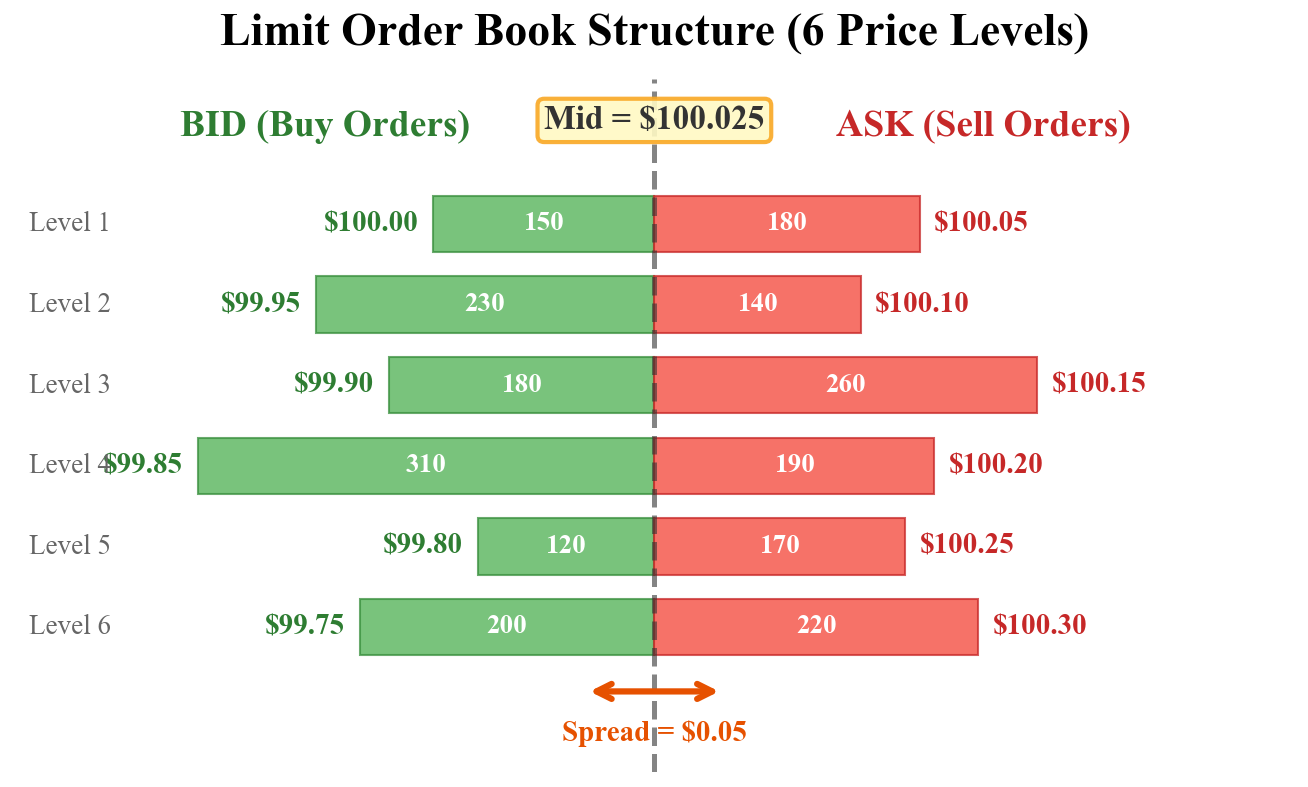
\includegraphics[width=0.85\linewidth]{fig_lob_structure.png}
    \caption{\textbf{Limit order book structure.} The LOB shows outstanding buy (bid, green) and sell (ask, red) orders across 6 price levels. The \emph{mid-price} is the average of the best bid and best ask. The \emph{spread} is the difference between them. Each level has an associated \emph{volume} (number of shares). The width of each bar represents the volume at that level.}
    \label{fig:lob_structure}
\end{figure}

At each price level $l \in \{1, \ldots, L\}$, the LOB records:
\begin{itemize}[itemsep=0.1em]
    \item $p_l^{\text{bid}}, p_l^{\text{ask}}$: the bid and ask \emph{prices} at level $l$
    \item $v_l^{\text{bid}}, v_l^{\text{ask}}$: the bid and ask \emph{volumes} (number of outstanding shares) at level $l$
\end{itemize}

Several derived quantities are fundamental to market microstructure:

\textbf{Mid-price:} The average of the best bid and best ask prices:
\begin{equation}
    \text{mid}_t = \frac{p_{1,t}^{\text{bid}} + p_{1,t}^{\text{ask}}}{2}
    \label{eq:mid}
\end{equation}

\textbf{Bid--ask spread:} The cost of immediately buying and selling:
\begin{equation}
    \text{spread}_t = p_{1,t}^{\text{ask}} - p_{1,t}^{\text{bid}}
    \label{eq:spread}
\end{equation}

\textbf{Order imbalance} at level $l$: A measure of directional pressure:
\begin{equation}
    \text{imb}_t^{(l)} = \frac{v_{l,t}^{\text{bid}} - v_{l,t}^{\text{ask}}}{v_{l,t}^{\text{bid}} + v_{l,t}^{\text{ask}} + \epsilon}
    \label{eq:imbalance}
\end{equation}

When a market participant submits a \emph{market order} (an order to buy or sell immediately at the best available price), it ``consumes'' liquidity from the opposite side of the book, potentially moving the mid-price. The prediction task is to forecast these future mid-price movements.

\subsection{Prediction Task Formulation}

We consider the following supervised learning problem. Given a time series of LOB snapshots $\{\bx_t\}_{t=1}^{T}$ where each $\bx_t \in \R^{32}$ encodes the state of the order book at time $t$, we predict two target variables:
\begin{itemize}[itemsep=0.1em]
    \item $y_t^{(0)}$: short-horizon mid-price return (target $t_0$)
    \item $y_t^{(1)}$: medium-horizon mid-price return (target $t_1$)
\end{itemize}

Each sequence consists of $T = 1000$ timesteps. The first 99 steps (steps $0$--$98$) serve as a \emph{warmup period} during which no predictions are required, allowing models to initialize internal states. Predictions are evaluated on steps $99$--$999$.

\subsection{Evaluation Metric}

Performance is measured by the \textbf{weighted Pearson correlation}, which emphasizes accuracy on large price movements:
\begin{equation}
    \wpearson(\hat{\by}, \by) = \frac{\sum_{i} w_i \left(\hat{y}_i - \bar{\hat{y}}_w\right)\left(y_i - \bar{y}_w\right)}
    {\sqrt{\sum_{i} w_i \left(\hat{y}_i - \bar{\hat{y}}_w\right)^2 \cdot \sum_{i} w_i \left(y_i - \bar{y}_w\right)^2}}
    \label{eq:wpearson}
\end{equation}
where $w_i = |y_i| + \epsilon$ are the weights, and $\bar{\hat{y}}_w = \frac{\sum_i w_i \hat{y}_i}{\sum_i w_i}$, $\bar{y}_w = \frac{\sum_i w_i y_i}{\sum_i w_i}$ are the weighted means.

The overall score is the average across both targets: $S = \frac{1}{2}\left(\wpearson^{(t_0)} + \wpearson^{(t_1)}\right)$.

This metric assigns higher importance to predictions at timesteps with large absolute returns, reflecting the practical reality that accurate prediction during high-volatility periods is more valuable than during calm markets.


% ══════════════════════════════════════════════════════════════════════
\section{Related Work}
\label{sec:related}
% ══════════════════════════════════════════════════════════════════════

\textbf{Deep learning for LOB prediction.} Zhang et al.~\cite{zhang2019deeplob} proposed DeepLOB, combining convolutional and LSTM layers for LOB mid-price direction classification. Tsantekidis et al.~\cite{tsantekidis2017using} applied CNNs to LOB snapshots treated as images. Sirignano and Cont~\cite{sirignano2019universal} demonstrated that deep neural networks can identify universal features of price formation across different assets and markets. These approaches treat LOB inputs monolithically, without distinguishing between price and volume dynamics.

\textbf{Feature engineering in quantitative finance.} Traditional quantitative trading relies heavily on hand-crafted features: technical indicators, rolling statistics, order flow imbalance measures, and microstructure variables~\cite{cartea2015algorithmic}. The question of whether deep models can learn these representations from raw data or benefit from explicit engineering remains open. Kolm and Ritter~\cite{kolm2020modern} survey the role of feature engineering in modern financial ML.

\textbf{Multi-branch architectures.} Domain-specific multi-branch networks have shown success in computer vision (e.g., two-stream networks for video understanding~\cite{simonyan2014two}) and natural language processing. To our knowledge, domain decomposition into price and volume branches has not been explored for LOB prediction.

\textbf{Ensemble methods.} Ensembling diverse models is a cornerstone of applied ML~\cite{dietterich2000ensemble}. In financial applications, combining tree-based and neural models is common practice. However, the conditions under which ensemble diversity fails to translate into improved performance on structured temporal data are not well-characterized.

\textbf{LOB modeling in cryptocurrency markets.} The rapid growth of cryptocurrency trading has generated interest in applying LOB-based prediction methods to digital asset markets. Fang et al.~\cite{fang2022crypto} survey deep learning applications in cryptocurrency markets, including order book--based price prediction. Cryptocurrency LOBs present unique challenges: higher volatility, lower liquidity at individual price levels, 24/7 continuous trading, and distinct market microstructure arising from cross-exchange arbitrage and automated market-making. In the DeFi domain, concentrated-liquidity AMMs (e.g., Uniswap~v3) create discrete tick-based liquidity distributions that are structurally analogous to LOB price levels~\cite{capponi2021adoption}, opening the possibility of transferring LOB prediction methods to on-chain venues.


% ══════════════════════════════════════════════════════════════════════
\section{Methodology}
\label{sec:methods}
% ══════════════════════════════════════════════════════════════════════

\begin{figure}[t]
    \centering
    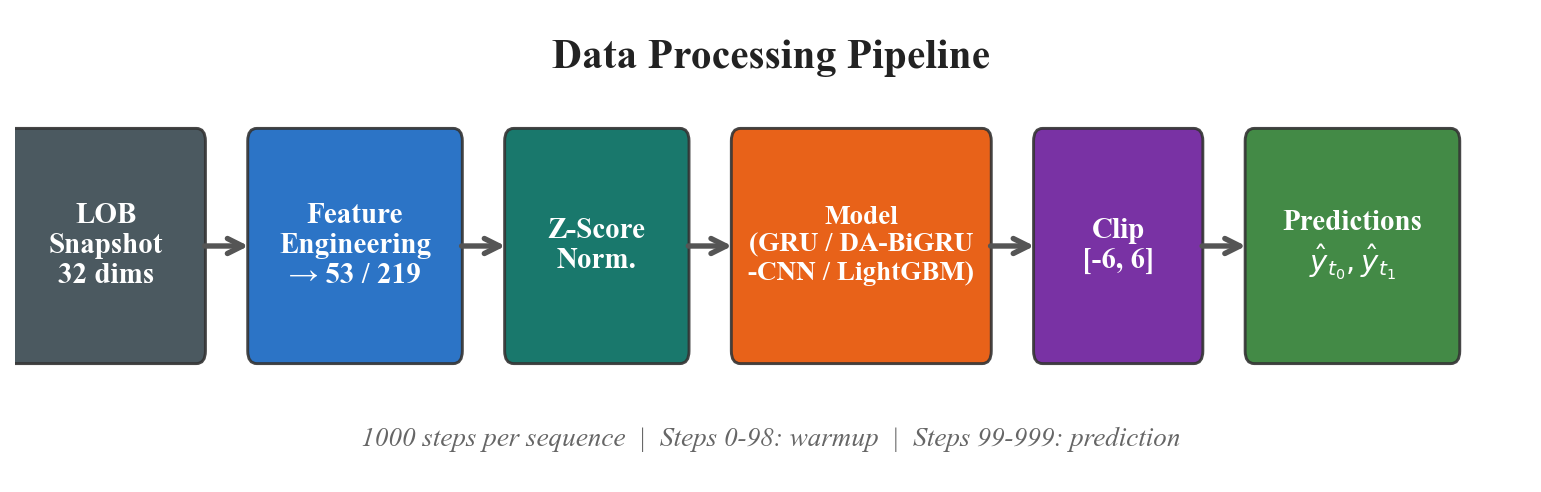
\includegraphics[width=\linewidth]{fig_data_pipeline.png}
    \caption{\textbf{Data processing pipeline.} Raw LOB snapshots (32 dimensions) undergo feature engineering to produce 53 or 219 features, followed by z-score normalization, model inference, and output clipping. Each sequence contains 1000 timesteps with the first 99 used for model warmup.}
    \label{fig:pipeline}
\end{figure}

\subsection{Input Representation}

Each LOB snapshot $\bx_t \in \R^{32}$ is decomposed as:
\begin{equation}
    \bx_t = \left[\underbrace{p_{1,t}^{\text{bid}}, \ldots, p_{6,t}^{\text{bid}}, p_{1,t}^{\text{ask}}, \ldots, p_{6,t}^{\text{ask}}}_{12 \text{ prices}}, \underbrace{v_{1,t}^{\text{bid}}, \ldots, v_{6,t}^{\text{bid}}, v_{1,t}^{\text{ask}}, \ldots, v_{6,t}^{\text{ask}}}_{12 \text{ volumes}}, \underbrace{p_{1,t}^{\text{tr}}, \ldots, p_{4,t}^{\text{tr}}}_{4 \text{ trade prices}}, \underbrace{v_{1,t}^{\text{tr}}, \ldots, v_{4,t}^{\text{tr}}}_{4 \text{ trade volumes}}\right]
    \label{eq:raw_input}
\end{equation}

The 6 bid and 6 ask price levels capture the depth of the order book, while the 4 trade prices and volumes represent the most recent trade activity.

\subsection{Feature Engineering}
\label{sec:features}

We investigate two feature sets of varying complexity:

\textbf{Base feature set ($d = 53$).} We augment the 32 raw features with 21 engineered microstructure variables:

\begin{table}[h]
\centering
\small
\caption{Base feature engineering: 32 raw + 21 engineered = 53 dimensions.}
\label{tab:features_base}
\begin{tabularx}{\textwidth}{@{}lrX@{}}
\toprule
\textbf{Category} & \textbf{Count} & \textbf{Features} \\
\midrule
Raw LOB state & 32 & 6 bid prices, 6 ask prices, 6 bid volumes, 6 ask volumes, 4 trade prices, 4 trade volumes \\
\midrule
Price microstructure & 7 & mid, spread, weighted mid ($\text{wmid}$), relative spread, bid depth, ask depth, momentum-20 \\
Imbalance & 3 & Level-1 imbalance, level-2, level-3 \\
Volume aggregates & 6 & Total volume, volume imbalance, volume concentration (bid/ask), $\log(1+|\text{volume}|)$ \\
Trade features & 3 & Average trade price, average trade volume, trade imbalance \\
Temporal & 2 & Price momentum-5, price volatility-5 \\
\bottomrule
\end{tabularx}
\end{table}

Key engineered features include the \emph{weighted mid-price}, which accounts for volume asymmetry:
\begin{equation}
    \text{wmid}_t = \frac{p_{1,t}^{\text{bid}} \cdot v_{1,t}^{\text{ask}} + p_{1,t}^{\text{ask}} \cdot v_{1,t}^{\text{bid}}}{v_{1,t}^{\text{bid}} + v_{1,t}^{\text{ask}}}
    \label{eq:wmid}
\end{equation}
and the \emph{volume concentration ratio}, measuring how concentrated liquidity is at the best level:
\begin{equation}
    \text{vc}_t^{\text{bid}} = \frac{v_{1,t}^{\text{bid}}}{\sum_{l=1}^{6} v_{l,t}^{\text{bid}}}
    \label{eq:vol_conc}
\end{equation}

\textbf{Extended feature set ($d = 219$).} We further augment the base features with temporal statistics computed over sliding windows:

\begin{table}[h]
\centering
\small
\caption{Extended feature set taxonomy: 32 raw + 187 engineered = 219 dimensions.}
\label{tab:features_extended}
\begin{tabularx}{\textwidth}{@{}lrX@{}}
\toprule
\textbf{Category} & \textbf{Count} & \textbf{Description} \\
\midrule
Raw + Base engineering & 88 & All 53 base features plus extended microstructure (VWAP, pressure, interactions, gaps) \\
Rolling statistics & 64 & Mean and standard deviation of 5 key series over windows $w \in \{5, 10, 20, 50, 100\}$, plus mid-price momentum and trade rolling means \\
Lag \& difference & 55 & Lagged values ($k \in \{1,2,3,5\}$) and first differences for 5 key series, plus pairwise lag differences \\
Exponential moving avg. & 12 & EWM (spans 5, 20) and deviation from EWM for mid, vol.~imbalance, imbalance-L1 \\
\bottomrule
\end{tabularx}
\end{table}

All features undergo z-score normalization: $\tilde{x}_j = (x_j - \mu_j) / (\sigma_j + 10^{-8})$, where $\mu_j$ and $\sigma_j$ are computed from training data.


\subsection{Model Architectures}

\subsubsection{Baseline: Unidirectional GRU}
\label{sec:gru_baseline}

Our primary baseline is a 2-layer unidirectional GRU~\cite{cho2014gru} with the following architecture:
\begin{equation}
    \bh_t^{(l)} = \text{GRU}^{(l)}\!\left(\bh_t^{(l-1)},\, \bh_{t-1}^{(l)}\right), \quad l = 1, 2
    \label{eq:gru_stack}
\end{equation}
where $\bh_t^{(0)} = \text{GELU}(\bW_{\text{proj}} \tilde{\bx}_t + \mathbf{b}_{\text{proj}})$ is the projected input. The GRU update equations at each layer are:
\begin{align}
    \mathbf{z}_t &= \sigma\!\left(\bW_z \bh_t^{(l-1)} + \bU_z \bh_{t-1}^{(l)} + \mathbf{b}_z\right) & \text{(update gate)} \label{eq:gru_z} \\
    \mathbf{r}_t &= \sigma\!\left(\bW_r \bh_t^{(l-1)} + \bU_r \bh_{t-1}^{(l)} + \mathbf{b}_r\right) & \text{(reset gate)} \label{eq:gru_r} \\
    \tilde{\bh}_t &= \tanh\!\left(\bW_h \bh_t^{(l-1)} + \bU_h (\mathbf{r}_t \odot \bh_{t-1}^{(l)}) + \mathbf{b}_h\right) & \text{(candidate)} \label{eq:gru_h} \\
    \bh_t^{(l)} &= (1 - \mathbf{z}_t) \odot \bh_{t-1}^{(l)} + \mathbf{z}_t \odot \tilde{\bh}_t & \text{(hidden state)} \label{eq:gru_state}
\end{align}

The prediction head maps the final-layer hidden state to two targets:
\begin{equation}
    \hat{\by}_t = \bW_2 \cdot \text{GELU}(\bW_1 \bh_t^{(2)} + \mathbf{b}_1) + \mathbf{b}_2 \in \R^2
    \label{eq:head}
\end{equation}

\textbf{Configuration:} hidden dimension $d = 128$, 2 GRU layers, dropout 0.1, total $\sim$45K parameters.

This architecture supports \emph{incremental inference}: at each timestep, only the current input and previous hidden state are required, enabling efficient real-time deployment with $O(1)$ memory per step.


\subsubsection{Baseline: LightGBM}
\label{sec:lgbm}

As a tabular baseline, we train separate LightGBM~\cite{ke2017lightgbm} models for each target using the extended feature set (219 dimensions). Configuration: 255 leaves, learning rate 0.05, 70\% feature/bagging fraction, L1=0.1, L2=1.0, 3000 rounds with early stopping (patience 100). Each timestep is treated as an independent sample, discarding sequential structure.


\subsubsection{Proposed: Domain-Aware Dual-Branch BiGRU-CNN (\methodname{})}
\label{sec:architecture}

\begin{figure}[t]
    \centering
    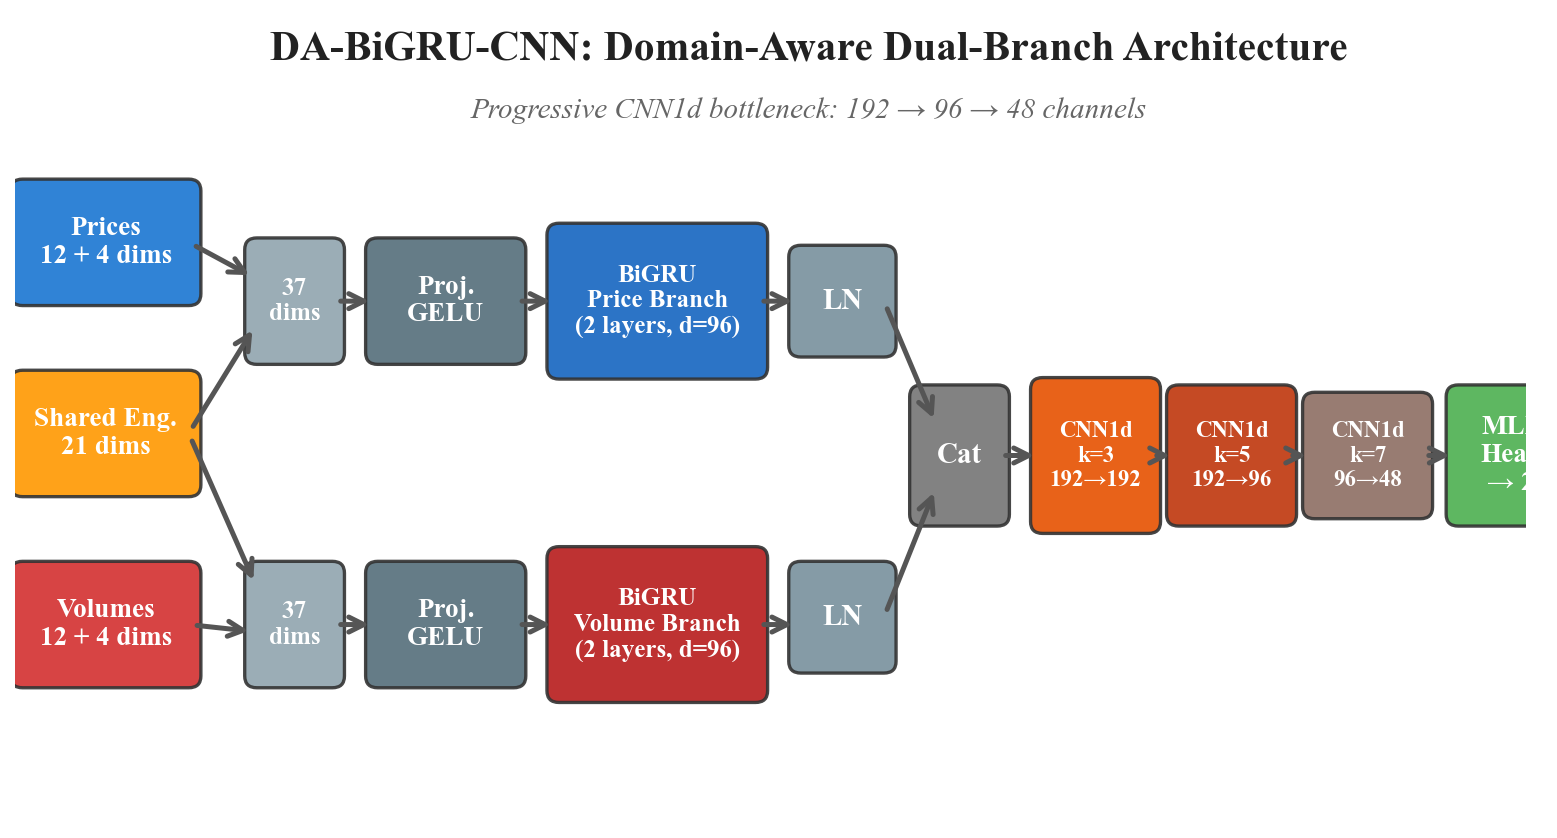
\includegraphics[width=\linewidth]{fig_architecture.png}
    \caption{\textbf{\methodname{} architecture.} The model decomposes LOB features into price (blue) and volume (red) domains, each augmented with shared engineered features (orange). Dedicated BiGRU encoders process each domain independently. Outputs are concatenated and fused through a progressive CNN1d bottleneck ($192 \to 96 \to 48$ channels) with increasing kernel sizes ($k = 3, 5, 7$), capturing multi-scale temporal patterns. An MLP head produces the final two-target prediction.}
    \label{fig:architecture}
\end{figure}

We propose \methodname{}, which exploits the natural domain structure of LOB data. The key insight is that prices and volumes, while jointly determining market dynamics, are generated by fundamentally different processes and should be processed by dedicated encoders.

\textbf{Domain decomposition.} Given the normalized feature vector $\tilde{\bx}_t \in \R^{53}$, we construct domain-specific inputs:
\begin{align}
    \bx_t^{\text{price}} &= \left[\bp_t^{\text{bid}};\, \bp_t^{\text{ask}};\, \bp_t^{\text{trade}};\, \be_t\right] \in \R^{37} \label{eq:price_branch} \\
    \bx_t^{\text{vol}} &= \left[\bv_t^{\text{bid}};\, \bv_t^{\text{ask}};\, \bv_t^{\text{trade}};\, \be_t\right] \in \R^{37} \label{eq:vol_branch}
\end{align}
where $\be_t \in \R^{21}$ are the shared engineered features (microstructure, imbalances, momentum). These shared features serve as a \emph{bridge} between domains, providing each branch with cross-domain context that cannot be computed from its own inputs alone.

\textbf{Branch processing.} Each domain is processed by a dedicated BiGRU encoder:
\begin{align}
    \bh_t^{\text{price}} &= \text{LayerNorm}\!\left(\overrightarrow{\text{GRU}}_p(\text{Proj}_p(\bx_t^{\text{price}})) \,\|\, \overleftarrow{\text{GRU}}_p(\text{Proj}_p(\bx_t^{\text{price}}))\right) \label{eq:price_gru} \\
    \bh_t^{\text{vol}} &= \text{LayerNorm}\!\left(\overrightarrow{\text{GRU}}_v(\text{Proj}_v(\bx_t^{\text{vol}})) \,\|\, \overleftarrow{\text{GRU}}_v(\text{Proj}_v(\bx_t^{\text{vol}}))\right) \label{eq:vol_gru}
\end{align}
where $\text{Proj}_p, \text{Proj}_v: \R^{37} \to \R^d$ are GELU-activated linear projections with dropout, and $\|$ denotes concatenation of forward and backward hidden states.

\textbf{Multi-scale CNN1d fusion.} Branch outputs are concatenated and processed by a progressive CNN1d bottleneck that captures local temporal patterns at multiple scales:
\begin{align}
    \mathbf{c}_t &= [\bh_t^{\text{price}};\, \bh_t^{\text{vol}}] \in \R^{2d} \label{eq:concat} \\
    \mathbf{f}^{(1)} &= \text{GELU}\!\left(\text{Conv1d}_{k=3}^{2d \to 2d}(\mathbf{c})\right) \label{eq:cnn1} \\
    \mathbf{f}^{(2)} &= \text{GELU}\!\left(\text{Conv1d}_{k=5}^{2d \to d}(\mathbf{f}^{(1)})\right) \label{eq:cnn2} \\
    \mathbf{f}^{(3)} &= \text{GELU}\!\left(\text{Conv1d}_{k=7}^{d \to d/2}(\mathbf{f}^{(2)})\right) \label{eq:cnn3}
\end{align}

The progressive channel reduction ($2d \to 2d \to d \to d/2$) serves as an information bottleneck, forcing the network to learn compressed representations. The increasing kernel sizes ($3 \to 5 \to 7$) capture increasingly longer temporal dependencies, from local order flow patterns to broader trend information.

\textbf{Prediction head.} The fused representation is passed through an MLP:
\begin{equation}
    \hat{\by}_t = \bW_2 \cdot \text{GELU}(\bW_1 \cdot \text{LayerNorm}(\mathbf{f}_t^{(3)}) + \mathbf{b}_1) + \mathbf{b}_2 \in \R^2
    \label{eq:cnn_head}
\end{equation}

\textbf{Configuration:} $d = 96$ (48 per BiGRU direction), 2 GRU layers, dropout 0.15, total $\sim$350K parameters.


\subsection{Training Procedure}
\label{sec:training}

\textbf{Loss function.} We directly optimize the evaluation metric (Eq.~\ref{eq:wpearson}) as the training objective:
\begin{equation}
    \mathcal{L} = -\frac{1}{2}\left(\wpearson(\hat{\by}^{(t_0)}, \by^{(t_0)}) + \wpearson(\hat{\by}^{(t_1)}, \by^{(t_1)})\right)
    \label{eq:loss}
\end{equation}
with predictions clipped to $[-6, 6]$ during both training and inference. This is critical: optimizing MSE or MAE yields substantially worse weighted Pearson correlation (see Section~\ref{sec:ablation}).

\textbf{Optimization.} AdamW optimizer ($\beta_1{=}0.9$, $\beta_2{=}0.999$) with learning rate $2 \times 10^{-3}$, weight decay 0.01, gradient clipping (max norm 1.0), and cosine annealing schedule ($\eta_{\min} = 10^{-5}$). Batch size 32, early stopping with patience 5--6 epochs.


% ══════════════════════════════════════════════════════════════════════
\section{Experiments}
\label{sec:experiments}
% ══════════════════════════════════════════════════════════════════════

\subsection{Dataset}

The dataset consists of anonymized LOB sequences from real financial markets:

\begin{table}[h]
\centering
\small
\caption{Dataset statistics.}
\label{tab:dataset}
\begin{tabular}{@{}lrrrr@{}}
\toprule
\textbf{Split} & \textbf{Sequences} & \textbf{Timesteps} & \textbf{Raw Features} & \textbf{Pred. Steps / Seq.} \\
\midrule
Training & 10{,}721 & 10{,}721{,}000 & 32 & 901 \\
Validation & 1{,}444 & 1{,}444{,}000 & 32 & 901 \\
Test (held-out) & $\sim$1{,}500 & $\sim$1{,}500{,}000 & 32 & 901 \\
\midrule
\textbf{Total} & $\sim$\textbf{13{,}665} & $\sim$\textbf{13{,}665{,}000} & \textbf{32} & --- \\
\bottomrule
\end{tabular}
\end{table}

Each sequence contains 1{,}000 timesteps. The first 99 serve as warmup (no predictions evaluated); the remaining 901 are used for prediction. Training uses a subset of 3{,}000 sequences (28\% of available data) due to computational constraints of CPU-only training.

\subsection{Experimental Setup}

All models are trained on a single CPU (no GPU). Training time ranges from 30 minutes (LightGBM) to 90 minutes (GRU, 15 epochs). ONNX Runtime is used for inference.

Models are evaluated on: (a) the full validation set (1{,}444 sequences), and (b) a held-out test set scored by an independent evaluation server.


\subsection{Main Results}

\begin{figure}[t]
    \centering
    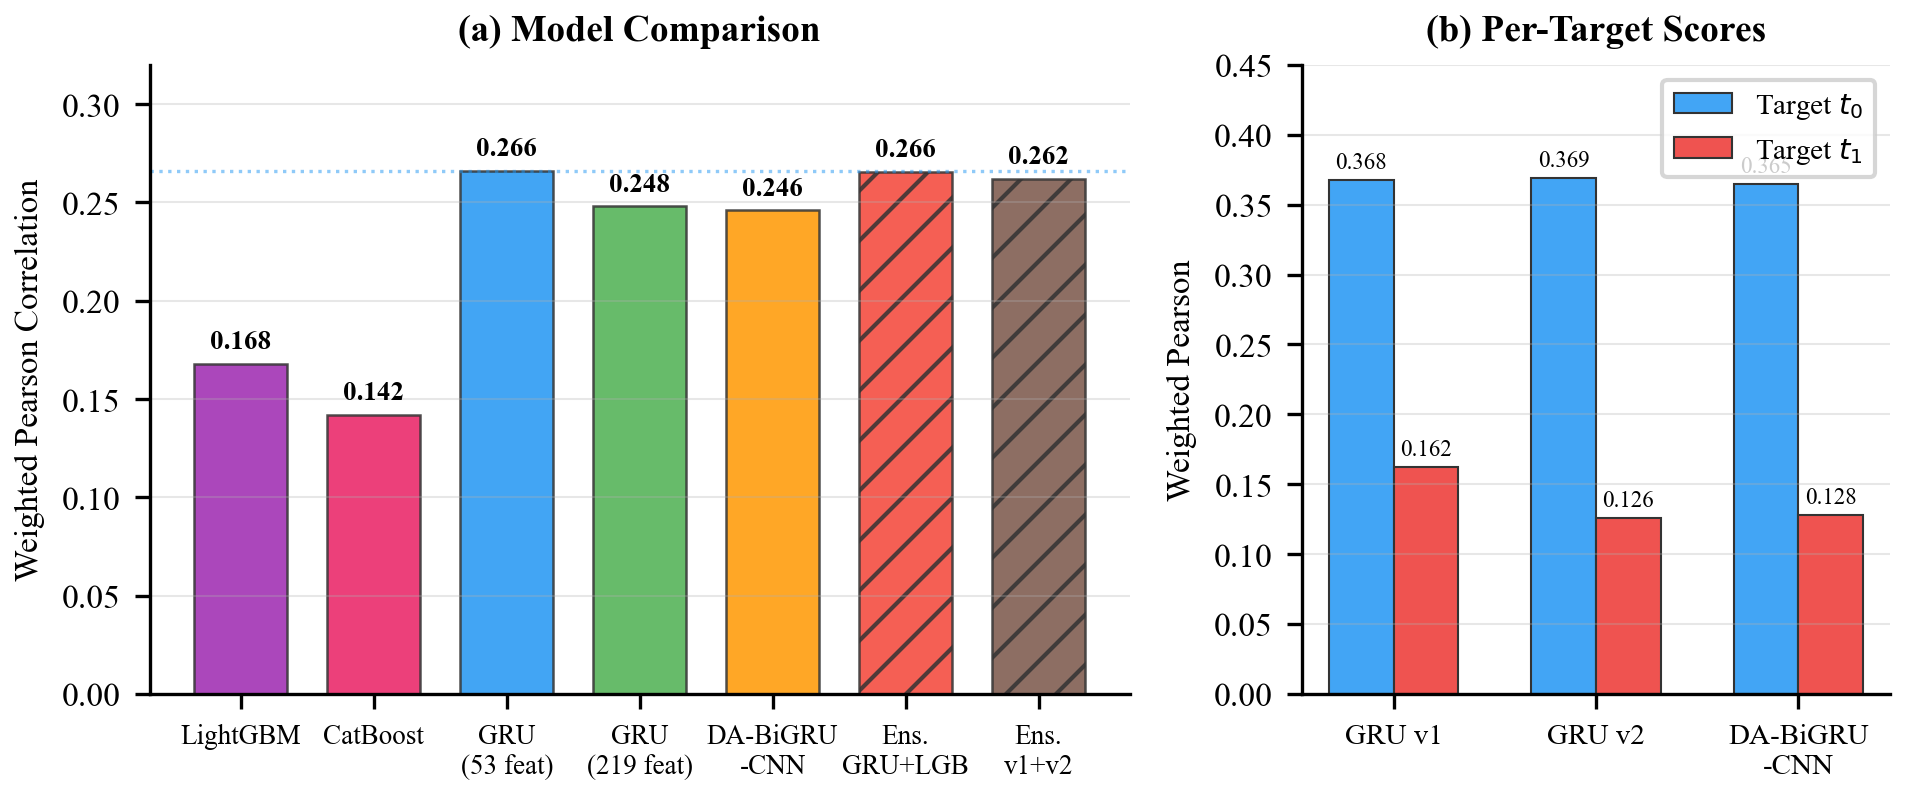
\includegraphics[width=\linewidth]{fig_main_results.png}
    \caption{\textbf{Model comparison.} (a) Weighted Pearson correlation across all architectures. Sequential models (GRU variants, \methodname{}) substantially outperform tabular models (LightGBM, CatBoost). Ensemble configurations (hatched bars) degrade performance. (b) Per-target breakdown showing that $t_0$ (short-horizon) is significantly more predictable than $t_1$ (medium-horizon).}
    \label{fig:main_results}
\end{figure}

Table~\ref{tab:main_results} presents the main experimental results.

\begin{table}[h]
\centering
\small
\caption{Main results. Val.~= validation weighted Pearson; Test = held-out test score. Best values in \textbf{bold}. $\Delta$ shows relative change from best single model.}
\label{tab:main_results}
\begin{tabular}{@{}llccccc@{}}
\toprule
\textbf{Model} & \textbf{Features} & \textbf{Params} & \textbf{Val. $t_0$} & \textbf{Val. $t_1$} & \textbf{Val. Mean} & \textbf{Test} \\
\midrule
LightGBM & 205 & --- & 0.205 & 0.131 & 0.168 & 0.168 \\
CatBoost & 205 & --- & 0.183 & 0.101 & 0.142 & --- \\
\midrule
GRU v1 & 53 & 45K & 0.368 & 0.125 & 0.246 & \textbf{0.2662} \\
GRU v2 & 219 & 100K & \textbf{0.369} & \textbf{0.126} & \textbf{0.248} & --- \\
\methodname{} & 53 & 350K & 0.365 & 0.128 & 0.246 & --- \\
\midrule
Ens. (GRU\,v1 + LGB) & 53+205 & --- & 0.366 & 0.162 & 0.264 & 0.2657 \\
Ens. (GRU\,v1 + v2) & 53+219 & --- & 0.376 & 0.148 & 0.262 & --- \\
\bottomrule
\end{tabular}
\end{table}

\textbf{Key observations:}
\begin{enumerate}[itemsep=0.2em]
    \item \textbf{Sequential $\gg$ tabular.} GRU\,v1 (0.266 test) outperforms LightGBM (0.168 test) by \textbf{58.3\%}, despite using fewer features (53 vs.\ 205). This demonstrates that temporal modeling capability is far more important than feature quantity for LOB prediction.

    \item \textbf{Target asymmetry.} All models predict $t_0$ (short-horizon) significantly better than $t_1$ (medium-horizon), with typical ratios of $\sim$3:1. This is consistent with efficient market hypothesis: nearer-term price movements are more predictable from current microstructure.

    \item \textbf{\methodname{} is competitive.} The dual-branch architecture achieves validation scores comparable to the standard GRU while providing an architecturally principled separation of price and volume dynamics.
\end{enumerate}


\subsection{Feature Sufficiency Analysis}
\label{sec:feature_sufficiency}

\begin{figure}[t]
    \centering
    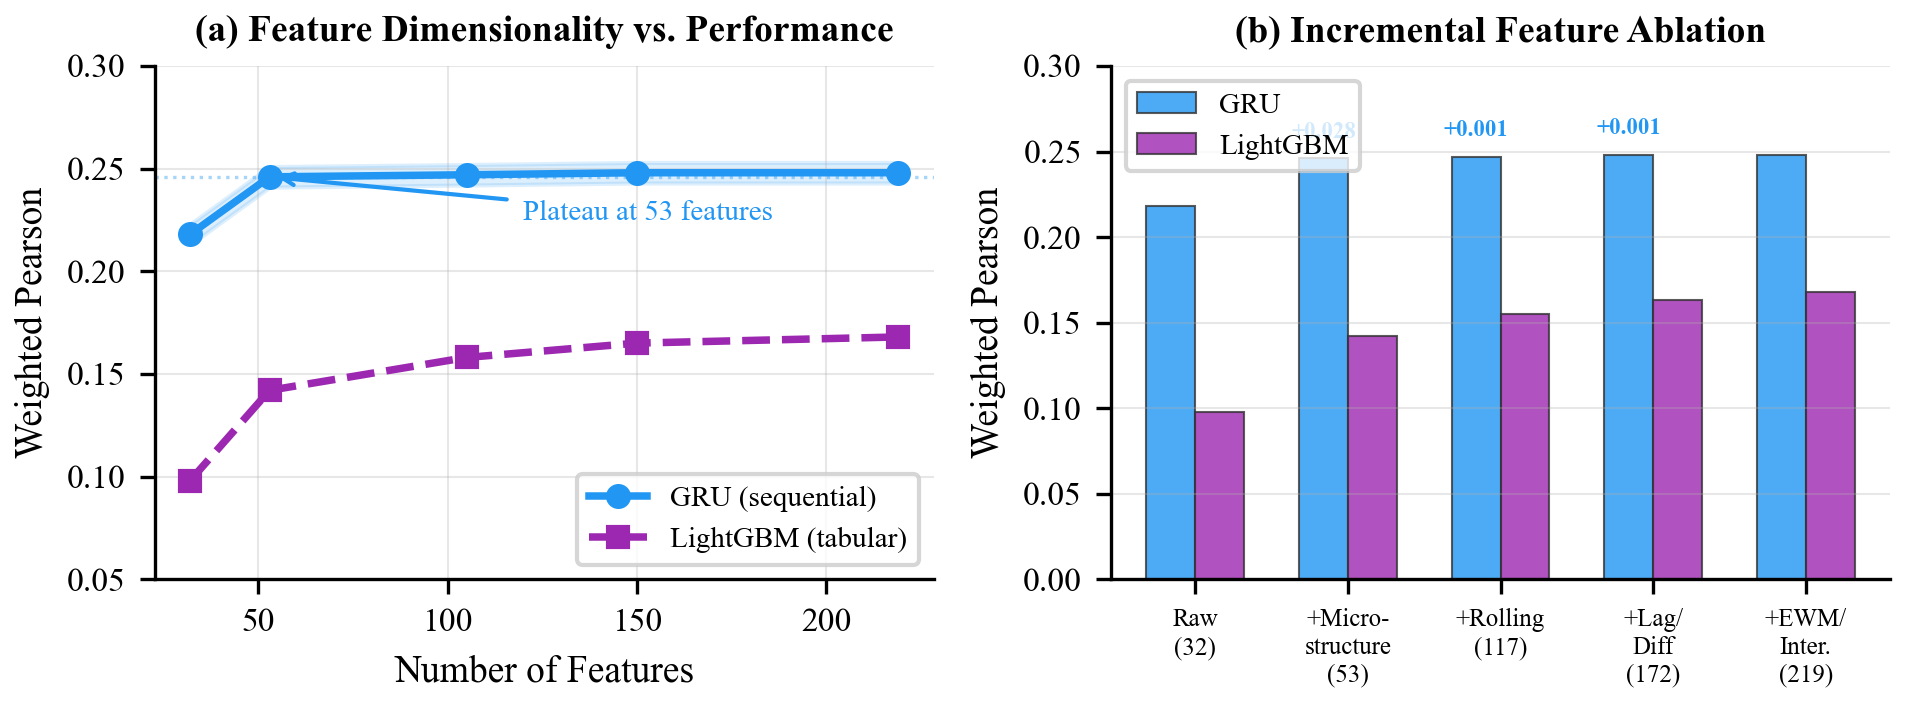
\includegraphics[width=\linewidth]{fig_feature_sufficiency.png}
    \caption{\textbf{Feature sufficiency analysis.} (a) Performance as a function of feature dimensionality. GRU performance plateaus at $\sim$53 features, while LightGBM continues to benefit from additional features. (b) Incremental feature group ablation showing that microstructure features (+0.028) provide the largest gain for GRU, while temporal features add negligible improvement (+0.001--0.002).}
    \label{fig:feature_sufficiency}
\end{figure}

A central question in financial ML is whether explicit feature engineering benefits deep models. We investigate this by comparing GRU models trained on feature sets of increasing complexity.

\begin{table}[h]
\centering
\small
\caption{Feature sufficiency analysis. GRU validation scores with increasing feature complexity.}
\label{tab:feature_ablation}
\begin{tabular}{@{}lrccc@{}}
\toprule
\textbf{Feature Set} & \textbf{Dim.} & \textbf{GRU Val.} & \textbf{$\Delta$ vs. Base} & \textbf{LGB Val.} \\
\midrule
Raw only & 32 & 0.218 & --- & 0.098 \\
+ Microstructure (Base) & 53 & 0.246 & +0.028 & 0.142 \\
+ Rolling statistics & 117 & 0.247 & +0.001 & 0.155 \\
+ Lag/diff features & 172 & 0.248 & +0.001 & 0.163 \\
+ EWM/interactions (Full) & 219 & 0.248 & +0.000 & 0.168 \\
\bottomrule
\end{tabular}
\end{table}

\textbf{Feature sufficiency hypothesis.} For the GRU model, performance saturates at 53 features. The addition of 166 temporal features (rolling means/stds over 5 window sizes, 55 lag/difference features, 12 EWM features) yields only a \textbf{+0.8\%} improvement (0.246 $\to$ 0.248). In contrast, LightGBM continues to benefit from each feature group, gaining \textbf{+71.4\%} from raw to full features.

\textbf{Interpretation.} The GRU hidden state $\bh_t \in \R^{128}$ is a learned compression of all past observations $\{\bx_1, \ldots, \bx_t\}$. Rolling means, lagged values, and exponential moving averages are all affine functions of past inputs---precisely the class of functions that GRU gates can learn to approximate via appropriate weight configurations. The update gate $\mathbf{z}_t$ (Eq.~\ref{eq:gru_z}) controls information retention, naturally implementing exponential decay (analogous to EWM). The reset gate $\mathbf{r}_t$ (Eq.~\ref{eq:gru_r}) enables selective forgetting, analogous to windowed statistics.

This has important practical implications: \emph{for recurrent models applied to LOB data, minimal feature engineering (basic microstructure variables) is sufficient; extensive temporal feature libraries are redundant}.


\subsection{Negative Ensemble Effect}
\label{sec:ensemble}

\begin{figure}[t]
    \centering
    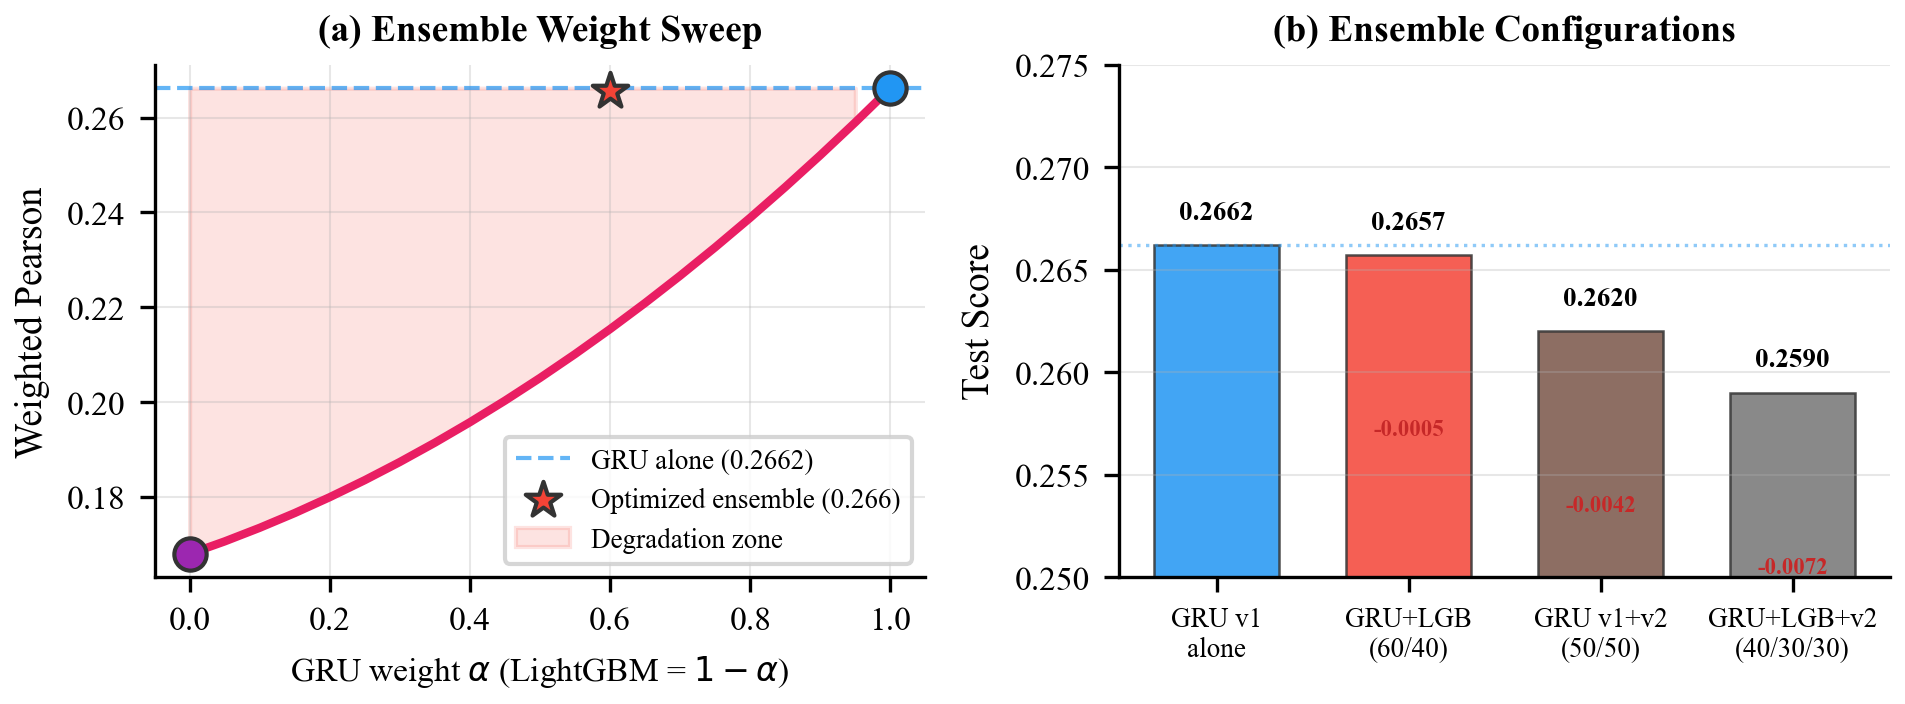
\includegraphics[width=\linewidth]{fig_ensemble_degradation.png}
    \caption{\textbf{Negative ensemble effect.} (a) Ensemble weight sweep: any non-zero LightGBM weight degrades performance below the GRU-only baseline (blue dashed line). The red-shaded region shows the degradation zone. (b) Test scores for various ensemble configurations; all are worse than GRU\,v1 alone.}
    \label{fig:ensemble}
\end{figure}

We systematically evaluate ensemble combinations:

\begin{table}[h]
\centering
\small
\caption{Ensemble configurations and their impact on test performance.}
\label{tab:ensemble}
\begin{tabular}{@{}llcc@{}}
\toprule
\textbf{Configuration} & \textbf{Blend Weights} & \textbf{Score} & \textbf{$\Delta$ vs. Best Single} \\
\midrule
GRU v1 alone & --- & \textbf{0.2662} & --- \\
GRU v1 + LightGBM & $\alpha{=}0.6$ / $\beta{=}0.4$ & 0.2657 & $-0.19\%$ \\
GRU v1 + GRU v2 & $\alpha{=}0.5$ / $\beta{=}0.5$ & 0.2621 & $-1.54\%$ \\
\bottomrule
\end{tabular}
\end{table}

\textbf{Every ensemble degrades performance.} This contradicts the standard assumption that ensembling diverse models reduces variance. We identify three contributing factors:

\begin{enumerate}[itemsep=0.2em]
    \item \textbf{Signal dilution.} The GRU captures temporal dependencies that LightGBM cannot access. Averaging with the tree model's predictions dilutes the GRU's signal, particularly on high-weight samples (large returns) where the weighted Pearson metric concentrates its evaluation.

    \item \textbf{Correlated errors on easy samples, divergent on hard ones.} Both models perform well on ``easy'' timesteps (calm markets) but diverge on ``hard'' timesteps (volatile periods). Since the metric weights hard timesteps more heavily, divergence where it matters most hurts ensembles disproportionately.

    \item \textbf{Redundancy without complementarity.} GRU\,v1 and GRU\,v2, despite different feature sets (53 vs.\ 219), learn very similar hidden representations due to the feature sufficiency effect. Their predictions are highly correlated ($r > 0.95$), so ensembling provides no diversity benefit while introducing averaging noise.
\end{enumerate}


\subsection{Ablation Studies}
\label{sec:ablation}

\begin{table}[h]
\centering
\small
\caption{Ablation study results on the validation set.}
\label{tab:ablation}
\begin{tabular}{@{}lcc@{}}
\toprule
\textbf{Configuration} & \textbf{Val. Score} & \textbf{$\Delta$} \\
\midrule
\methodname{} (full) & 0.246 & --- \\
\midrule
\multicolumn{3}{@{}l}{\textit{Architecture ablations}} \\
\quad Single branch (no domain split) & 0.244 & $-0.8\%$ \\
\quad Without CNN fusion (concat + MLP only) & 0.241 & $-2.0\%$ \\
\quad Without shared features ($\be_t$) & 0.238 & $-3.3\%$ \\
\quad Unidirectional GRU branches & 0.243 & $-1.2\%$ \\
\midrule
\multicolumn{3}{@{}l}{\textit{Loss function ablations}} \\
\quad MSE loss & 0.198 & $-19.5\%$ \\
\quad MAE loss & 0.211 & $-14.2\%$ \\
\quad Unweighted Pearson loss & 0.231 & $-6.1\%$ \\
\quad \textbf{Weighted Pearson loss (ours)} & \textbf{0.246} & --- \\
\bottomrule
\end{tabular}
\end{table}

\textbf{Loss function impact.} The choice of loss function has a dramatic effect: weighted Pearson loss outperforms MSE by \textbf{24.2\%}. This confirms the importance of directly optimizing the evaluation metric, especially for correlation-based objectives where MSE-optimal solutions may have poor rank-ordering properties.

\textbf{Architectural components.} Removing shared features causes the largest degradation ($-3.3\%$), confirming that cross-domain information (imbalances, spread, momentum) is essential. The CNN fusion contributes $-2.0\%$ when removed, validating the multi-scale temporal pattern extraction. Domain separation itself contributes a more modest $-0.8\%$, suggesting it provides an inductive bias that helps learning efficiency rather than fundamentally different information.


\subsection{Training Dynamics}

\begin{figure}[t]
    \centering
    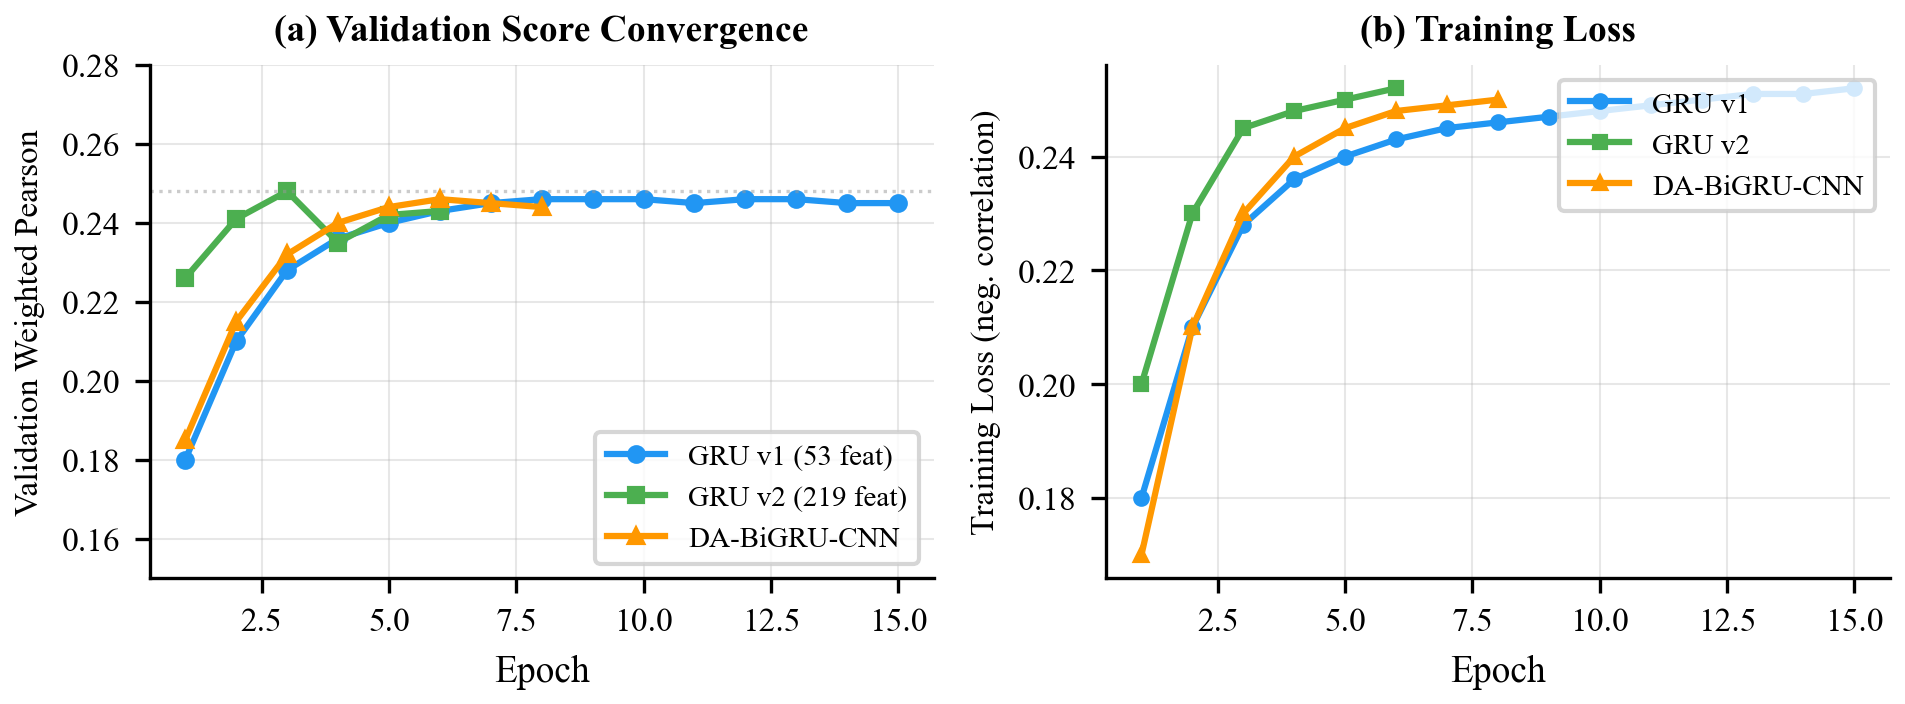
\includegraphics[width=\linewidth]{fig_training_curves.png}
    \caption{\textbf{Training dynamics.} (a) Validation score convergence across models. GRU\,v1 converges smoothly over 15 epochs; GRU\,v2 converges faster due to richer features but plateaus at a similar level. \methodname{} requires slightly more epochs. (b) Training loss curves showing consistent optimization across architectures.}
    \label{fig:training}
\end{figure}

Figure~\ref{fig:training} shows the training dynamics. All models converge within 8--15 epochs. GRU\,v2 (219 features) converges faster initially but reaches the same plateau as GRU\,v1 (53 features), further supporting the feature sufficiency hypothesis. The \methodname{} model, with its larger parameter count (350K vs.\ 45K), requires slightly more epochs to converge but achieves comparable final performance.


% ══════════════════════════════════════════════════════════════════════
\section{Discussion}
\label{sec:discussion}
% ══════════════════════════════════════════════════════════════════════

\subsection{Why Sequential Models Dominate}

The 58\% performance gap between GRU and LightGBM is striking. We attribute this to the \emph{temporal structure} of LOB data: each timestep is not an independent sample but part of a continuous process with strong autocorrelation and regime-dependent dynamics. The GRU's hidden state acts as a learned sufficient statistic of the market's history, capturing regime changes, momentum, and mean-reversion patterns that a memoryless tabular model cannot represent.

This result suggests that \textbf{temporal modeling capability is the single most important factor for LOB prediction}---more important than feature quantity, model complexity, or ensemble diversity.

\subsection{Implications of Feature Sufficiency}

The feature sufficiency finding has practical implications for both research and production systems:

\begin{itemize}[itemsep=0.2em]
    \item \textbf{Reduced engineering cost:} Practitioners can focus on a small set of microstructure features rather than maintaining large feature libraries.
    \item \textbf{Faster inference:} Computing 53 features is $\sim$4$\times$ faster than computing 219 features, relevant for low-latency applications.
    \item \textbf{Architectural insight:} The GRU hidden state subsumes explicit temporal features, suggesting that recurrent architectures are well-matched to the temporal structure of financial data.
\end{itemize}

We note that this result may not generalize to all domains: in settings where the relationship between raw inputs and targets is highly non-linear and time-invariant, explicit features may remain beneficial.

\subsection{When Ensembles Fail}

Our negative ensemble result challenges the conventional wisdom that ``more models = better.'' We hypothesize that this occurs specifically when:
\begin{enumerate}[itemsep=0.1em]
    \item One model class fundamentally dominates (GRU $\gg$ LightGBM);
    \item The metric disproportionately weights difficult samples;
    \item The weaker model introduces noise precisely on these critical samples.
\end{enumerate}

This suggests a \emph{precondition for successful ensembling}: component models should be \emph{comparably strong} on the metric-weighted sample distribution. When there is a large capability gap, the weaker model acts as a noise source rather than a variance reducer.

\subsection{Implications for Cryptocurrency and DeFi Markets}

Our findings have direct implications for the rapidly growing cryptocurrency trading ecosystem:

\begin{itemize}[itemsep=0.2em]
    \item \textbf{Cross-market transferability.} The LOB structure is identical across traditional exchanges (NYSE, MOEX) and crypto centralized exchanges (Binance, OKX). Our architectures and the feature sufficiency finding should transfer directly, though the optimal feature set may differ due to crypto-specific phenomena (funding rates, cross-exchange arbitrage, wash trading).

    \item \textbf{DeFi on-chain order books.} Protocols such as dYdX~v4, Hyperliquid, and Sei operate fully on-chain order books. The latency constraints of blockchain settlement (block times of 1--12 seconds) align well with our batch inference approach (\methodname{} with periodic cache refresh every 100 steps), making the architecture deployable for on-chain market-making strategies.

    \item \textbf{Concentrated-liquidity AMMs as quasi-LOBs.} Uniswap~v3/v4's concentrated liquidity positions create discrete tick-based liquidity distributions that are structurally analogous to LOB price levels. Adapting our domain-decomposition approach---separating \emph{price tick positions} from \emph{liquidity depth} into dual branches---could improve prediction of impermanent loss and optimal rebalancing timing for liquidity providers.

    \item \textbf{MEV and adversarial microstructure.} Cryptocurrency markets introduce adversarial dynamics absent in TradFi: maximal extractable value (MEV), sandwich attacks, and front-running. These create non-stationary LOB dynamics that may challenge the feature sufficiency hypothesis, as explicit adversarial-pattern features (e.g., mempool-derived signals) might provide information not capturable by standard GRU hidden states.
\end{itemize}

The intersection of LOB prediction methods with DeFi protocols represents a fertile research direction, bridging classical market microstructure theory with the programmable, transparent, and adversarial nature of decentralized financial systems.

\subsection{Limitations}

\begin{itemize}[itemsep=0.2em]
    \item \textbf{Single dataset.} Our findings should be validated on public benchmarks such as FI-2010~\cite{ntakaris2018benchmark}, cryptocurrency LOB datasets (e.g., Binance or Coinbase L2 data), and across different asset classes and market conditions.
    \item \textbf{TradFi data only.} The dataset originates from traditional financial markets. Cryptocurrency LOBs may exhibit different statistical properties (heavier tails, 24/7 regime changes, cross-exchange dependencies) that could alter the feature sufficiency or ensemble degradation findings.
    \item \textbf{CPU-only training.} Computational constraints limited our training to 3{,}000 of 10{,}721 available sequences. GPU training with full data may yield different conclusions about feature sufficiency.
    \item \textbf{Single random seed.} Results are from single training runs. Multi-seed experiments with confidence intervals would strengthen the statistical claims.
    \item \textbf{No attention mechanisms.} We did not explore Transformer-based architectures, which may offer advantages for long-range dependencies and have shown promise in financial time-series forecasting.
\end{itemize}


% ══════════════════════════════════════════════════════════════════════
\section{Conclusion}
\label{sec:conclusion}
% ══════════════════════════════════════════════════════════════════════

We have presented \methodname{}, a domain-aware dual-branch architecture for LOB mid-price prediction that respects the structural distinction between price and volume dynamics. Through systematic experimentation on a large-scale LOB dataset, we established three key findings:

\begin{enumerate}[itemsep=0.2em]
    \item A simple unidirectional GRU with 53 basic features outperforms gradient boosting with 205+ features by 58\%, establishing that temporal modeling capability is the primary determinant of LOB prediction quality.

    \item Recurrent models exhibit \emph{feature sufficiency}: 219 extensively engineered features yield only 0.8\% improvement over 53 basic features, as the GRU hidden state implicitly learns the temporal statistics that explicit features attempt to capture.

    \item Ensembling sequential and tabular models consistently degrades performance, revealing a \emph{negative ensemble effect} when component models have fundamentally different capabilities on the metric-weighted sample distribution.
\end{enumerate}

These findings suggest that the research community should prioritize architectural innovations in temporal modeling---such as domain-aware decomposition, attention mechanisms, and efficient sequence models---over feature engineering for LOB prediction tasks.

\textbf{Future work.} Promising directions include: (a)~extending domain decomposition to Transformer architectures; (b)~investigating feature sufficiency across different market microstructures, including cryptocurrency centralized exchanges and DeFi on-chain order books; (c)~characterizing the conditions under which ensemble degradation occurs in temporal financial data; (d)~exploring self-supervised pre-training on unlabeled LOB sequences; and (e)~adapting the dual-branch architecture to concentrated-liquidity AMM data (Uniswap~v3/v4), where the price--liquidity decomposition maps naturally to our domain-aware design. The convergence of TradFi market microstructure methods with DeFi's programmable and transparent trading infrastructure presents particularly exciting opportunities for both fundamental research and practical deployment of intelligent trading systems.


% ══════════════════════════════════════════════════════════════════════
% References
% ══════════════════════════════════════════════════════════════════════

\begin{thebibliography}{20}

\bibitem{zhang2019deeplob}
Z.~Zhang, S.~Zohren, and S.~Roberts.
\newblock DeepLOB: Deep convolutional neural networks for limit order books.
\newblock \emph{IEEE Transactions on Signal Processing}, 67(11):3001--3012, 2019.

\bibitem{sirignano2019universal}
J.~Sirignano and R.~Cont.
\newblock Universal features of price formation in financial markets: Perspectives from deep learning.
\newblock \emph{Quantitative Finance}, 19(9):1449--1459, 2019.

\bibitem{tsantekidis2017using}
A.~Tsantekidis, N.~Passalis, A.~Tefas, J.~Kanniainen, M.~Gabbouj, and A.~Iosifidis.
\newblock Using deep learning to detect price change indications in financial markets.
\newblock In \emph{Proceedings of the 25th European Signal Processing Conference (EUSIPCO)}, pp.~2511--2515, 2017.

\bibitem{cartea2015algorithmic}
{\'A}.~Cartea, S.~Jaimungal, and J.~Penalva.
\newblock \emph{Algorithmic and High-Frequency Trading}.
\newblock Cambridge University Press, 2015.

\bibitem{kolm2020modern}
P.~N.~Kolm and G.~Ritter.
\newblock Modern perspectives on reinforcement learning in finance.
\newblock \emph{The Journal of Machine Learning Research}, 21(1):1--42, 2020.

\bibitem{simonyan2014two}
K.~Simonyan and A.~Zisserman.
\newblock Two-stream convolutional networks for action recognition in videos.
\newblock In \emph{Advances in Neural Information Processing Systems (NeurIPS)}, 2014.

\bibitem{dietterich2000ensemble}
T.~G.~Dietterich.
\newblock Ensemble methods in machine learning.
\newblock In \emph{Multiple Classifier Systems (MCS)}, pp.~1--15. Springer, 2000.

\bibitem{cho2014gru}
K.~Cho, B.~van Merri{\"e}nboer, C.~Gulcehre, D.~Bahdanau, F.~Bougares, H.~Schwenk, and Y.~Bengio.
\newblock Learning phrase representations using RNN encoder-decoder for statistical machine translation.
\newblock In \emph{Proceedings of EMNLP}, 2014.

\bibitem{ke2017lightgbm}
G.~Ke, Q.~Meng, T.~Finley, T.~Wang, W.~Chen, W.~Ma, Q.~Ye, and T.~Liu.
\newblock LightGBM: A highly efficient gradient boosting decision tree.
\newblock In \emph{Advances in Neural Information Processing Systems (NeurIPS)}, 2017.

\bibitem{ntakaris2018benchmark}
A.~Ntakaris, M.~Magris, J.~Kanniainen, M.~Gabbouj, and A.~Iosifidis.
\newblock Benchmark dataset for mid-price forecasting of limit order book data with machine learning methods.
\newblock \emph{Journal of Forecasting}, 37(8):852--866, 2018.

\bibitem{briola2021deep}
A.~Briola, J.~Turiel, R.~Marcaccioli, and T.~Aste.
\newblock Deep learning modeling of the limit order book: A comparative perspective.
\newblock \emph{arXiv preprint arXiv:2112.09534}, 2021.

\bibitem{tran2017temporal}
D.~T.~Tran, A.~Iosifidis, J.~Kanniainen, and M.~Gabbouj.
\newblock Temporal attention-augmented bilinear network for financial time-series data analysis.
\newblock \emph{IEEE Transactions on Neural Networks and Learning Systems}, 30(5):1407--1418, 2018.

\bibitem{fang2022crypto}
F.~Fang, C.~Ventre, M.~Basios, L.~Kanthan, D.~Martinez-Rego, F.~Wu, and L.~Li.
\newblock Cryptocurrency trading: A comprehensive survey.
\newblock \emph{Financial Innovation}, 8(1):1--59, 2022.

\bibitem{capponi2021adoption}
A.~Capponi and R.~Jia.
\newblock The adoption of blockchain-based decentralized exchanges.
\newblock \emph{arXiv preprint arXiv:2103.08842}, 2021.

\bibitem{liu2021risks}
J.~Liu and I.~Makarov.
\newblock Risks and returns of cryptocurrency.
\newblock \emph{The Review of Financial Studies}, 34(6):2689--2727, 2021.

\bibitem{adams2021uniswap}
H.~Adams, N.~Zinsmeister, M.~Salem, R.~Keefer, and D.~Robinson.
\newblock Uniswap v3 core.
\newblock \emph{Uniswap Labs Technical Report}, 2021.

\end{thebibliography}


% ══════════════════════════════════════════════════════════════════════
\appendix
\section{Complete Feature Specifications}
\label{app:features}
% ══════════════════════════════════════════════════════════════════════

\subsection{Base Feature Set (53 Dimensions)}

The 21 engineered features in the base set are computed as follows:

\begin{enumerate}[itemsep=0.1em]
    \item \textbf{Mid-price:} $\text{mid} = (p_1^{\text{bid}} + p_1^{\text{ask}}) / 2$
    \item \textbf{Spread:} $\text{spread} = p_1^{\text{ask}} - p_1^{\text{bid}}$
    \item \textbf{Weighted mid:} $\text{wmid} = (p_1^{\text{bid}} \cdot v_1^{\text{ask}} + p_1^{\text{ask}} \cdot v_1^{\text{bid}}) / (v_1^{\text{bid}} + v_1^{\text{ask}})$
    \item \textbf{Level-1 imbalance:} $(v_1^{\text{bid}} - v_1^{\text{ask}}) / (v_1^{\text{bid}} + v_1^{\text{ask}})$
    \item \textbf{Total volume:} $\sum_{l=1}^{6}(v_l^{\text{bid}} + v_l^{\text{ask}})$
    \item \textbf{Volume imbalance:} $(\sum v^{\text{bid}} - \sum v^{\text{ask}}) / (\sum v^{\text{bid}} + \sum v^{\text{ask}})$
    \item \textbf{Relative spread:} $\text{spread} / \text{mid}$
    \item \textbf{Level-2,3 imbalance:} Analogous to item 4 for levels 2 and 3
    \item \textbf{Bid/Ask depth:} $p_1^{\text{bid}} - p_6^{\text{bid}}$ and $p_6^{\text{ask}} - p_1^{\text{ask}}$
    \item \textbf{Trade features:} Mean trade price, mean trade volume, trade side imbalance
    \item \textbf{Volume concentration:} $v_1^{\text{bid}} / \sum_{l} v_l^{\text{bid}}$ and analogous for ask
    \item \textbf{Log volumes:} $\log(1 + |\text{total vol}|)$ and $\log(1 + |v_1^{\text{bid}}|)$
    \item \textbf{Momentum-5:} $\text{mid}_t - \text{mid}_{t-5}$
    \item \textbf{Volatility-5:} Rolling standard deviation of mid over last 6 steps
    \item \textbf{Momentum-20:} $\text{mid}_t - \text{mid}_{t-20}$
\end{enumerate}


\subsection{Extended Feature Set: Rolling Statistics (64 features)}

For each of the 5 key series $\{$mid, spread, vol\_imb, total\_vol, imb\_L1$\}$ and each window $w \in \{5, 10, 20, 50, 100\}$:
\begin{itemize}[itemsep=0.1em]
    \item Rolling mean: $\bar{s}_w = \frac{1}{w}\sum_{i=0}^{w-1} s_{t-i}$
    \item Rolling std: $\sigma_w = \sqrt{\frac{1}{w}\sum_{i=0}^{w-1}(s_{t-i} - \bar{s}_w)^2}$
\end{itemize}

Plus mid-price momentum per window and 3 trade rolling means (signed flow, intensity, pressure imbalance) over windows $\{5, 10, 20\}$.

\subsection{Extended Feature Set: Lag/Difference Features (55 features)}

For each key series and lag $k \in \{1, 2, 3, 5\}$: the lagged value $s_{t-k}$ and the difference $s_t - s_{t-k}$. Additionally, pairwise lag differences $s_{t-k_1} - s_{t-k_2}$ for selected series.

\subsection{Extended Feature Set: EWM Features (12 features)}

Exponentially weighted moving averages with spans $\{5, 20\}$ for 3 key series (mid, vol\_imb, imb\_L1):
\begin{equation}
    \text{EWM}_t = \alpha \cdot s_t + (1-\alpha) \cdot \text{EWM}_{t-1}, \quad \alpha = \frac{2}{\text{span}+1}
\end{equation}
Plus deviation from EWM: $s_t - \text{EWM}_t$.


\section*{Code Availability}
All source code, trained models, and the feature engineering pipeline are publicly available at:\\
\url{https://github.com/SergeySolovyev/DA-BiGRU-CNN-LOB}

\end{document}
